\documentclass[11pt, oneside]{article}   	% use "amsart" instead of "article" for AMSLaTeX format
\usepackage{geometry}                		% See geometry.pdf to learn the layout options. There are lots.
\geometry{letterpaper}                   		% ... or a4paper or a5paper or ... 
%\geometry{landscape}                		% Activate for for rotated page geometry
%\usepackage[parfill]{parskip}    		% Activate to begin paragraphs with an empty line rather than an indent
\usepackage{graphicx}				% Use pdf, png, jpg, or eps� with pdflatex; use eps in DVI mode
								% TeX will automatically convert eps --> pdf in pdflatex		
\usepackage{amssymb}
\usepackage{amsmath}
\usepackage{parskip}
\usepackage{color}
\usepackage{hyperref}

\title{Functions of a complex variable}
%\author{The Author}
%\section{}
%\subsection*{}
\date{}							% Activate to display a given date or no date

\graphicspath{{/Users/telliott_admin/Dropbox/Tex/png/}}
% \begin{center} 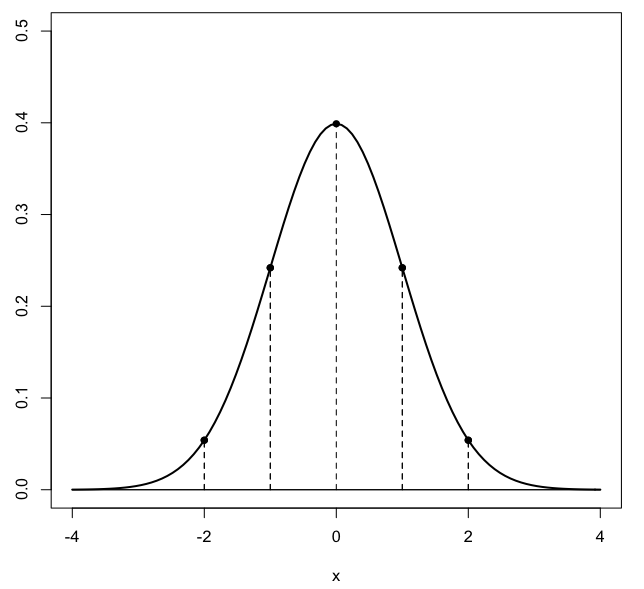
\includegraphics [scale=0.4] {gauss3.png} \end{center}
\begin{document}
\maketitle
\Large
\subsection*{conformal mapping}
At this point let's just remind ourselves how the visual representation of a complex function differs from the more familiar case of a function $f: \mathbb{R}^1  \rightarrow \mathbb{R}^1$.

In the real case, the first dimension is the independent variable $x$ and the second is $y=f(x)$ and the derivative is the \emph{slope} of the curve produced by plotting pairs of $x,f(x)$.

In the complex case, our numbers $z$ are points in the complex plane.  They are \emph{mapped} to other complex numbers in a different complex plane, which is often called $w$, where $w=f(z) = u(x,y) + i v(x,y)$.

The derivative does not have any notion of slope.  Our requirement for differentiability included the constraint that the derivative of the function at a point $z_0$ must be the same no matter from what direction we approach that point.  This leads to the CRE and the study of only analytic functions.  Many such functions may have isolated points at which they are not defined, and that will still be OK.

In the figure, is shown the mapping corresponding to the complex function $w = f(z) = z^2$.

\begin{center} 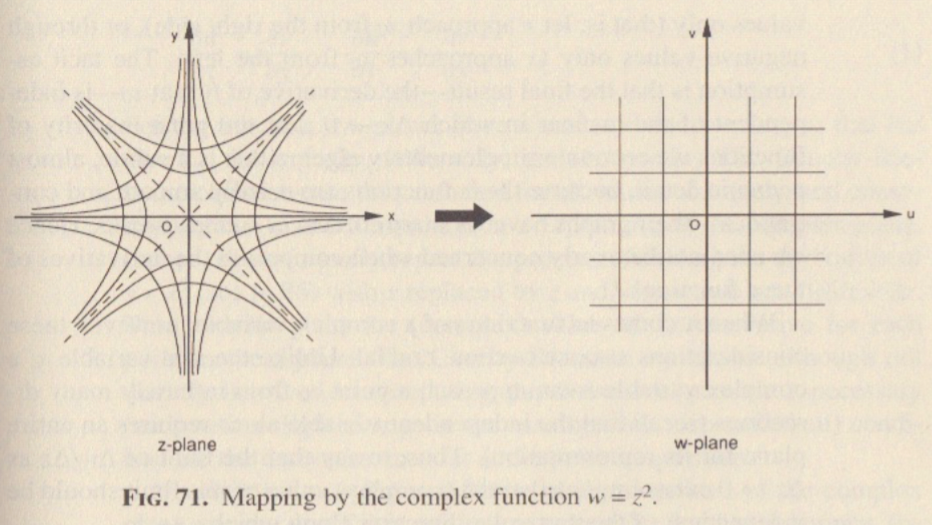
\includegraphics [scale=0.4] {zw-map.png} \end{center}

\[ z = x + iy \]
\[ z^2 = x^2 - y^2 + i2xy \]

The functions $u = x^2 - y^2$ and $v = 2xy$ are both hyperbolas.  Consider what happens in the case where $u = c$ where $c$ is a constant.  The values of $x$ and $y$ that satisfy this constrain lie on hyperbolas in the $z$-plane.  For example, the points on the curve $xy = 1/2$ correspond to the points on the curve $v=1$, which is a straight vertical line in the $w$ plane.

In this sense, the hyperbolic curves in the $z$-plane shown in the figure are mapped into rectangular grid in the $w$-plane.  An important note here is that the angles where these curves meet are the same in both the $z$-plane and the $w$-plane.  In both cases the lines meet at right angles.

According to wolfram

\url{http://mathworld.wolfram.com/ConformalMapping.html}

A conformal mapping, also called a \textbf{conformal map}, conformal transformation, angle-preserving transformation, or biholomorphic map, is a transformation that preserves local angles. An analytic function is conformal at any point where it has a nonzero derivative.

\subsection*{looking ahead}
As motivation to do the work that is coming, consider these statements from the summary article in wikipedia:

    One of the central tools in complex analysis is the line integral. The line integral around a closed path of a function that is holomorphic everywhere inside the area bounded by the closed path is always zero, which is what the Cauchy integral theorem states. The values of such a holomorphic function inside a disk can be computed by a path integral on the disk's boundary, as shown in (Cauchy's integral formula). 
    
    Path integrals in the complex plane are often used to determine complicated real integrals, and here the theory of residues among others is applicable (see methods of contour integration). A "pole" (or isolated singularity) of a function is a point where the function's value becomes unbounded, or "blows up". If a function has such a pole, then one can compute the function's residue there, which can be used to compute path integrals involving the function; this is the content of the powerful residue theorem.
    
\subsection*{harmonics}
Boas says this about analytic functions (that satisfy the CRE).

"If $f(z) = u = iv$ is analytic in a region, then $u$ and $v$ satisfy Laplace's equation, that is, $u$ and $v$ are harmonic functions..."

Laplace's equation is:

\[ \nabla^2 f = 0 \]

Consider the function 
\[ u(x,y) = x^2 - y^2 \]
\[ \nabla^2 u = \frac{\partial^2 u}{\partial x^2} +  \frac{\partial^2 u}{\partial y^2} \]
\[ = 2 - 2 = 0 \]

To find the function $v(x,y)$ such that $z = u + iv$ is analytic, use the CRE:
\[ u = x^2 - y^2 \]
\[ v_y = u_x = 2x \]
\[ v_x = - u_y = 2y \]
So it looks like $2xy$ will work.  In particular
\[ z = x^2 - y^2 + i2xy + \text{constant} \]

But of course 
\[  x^2 - y^2 + i2xy = (x + iy)^2 = z^2 \]
which does not depend on $z*$.

To explore why this is true, take the second derivatives of the CRE:
\[ u_x = v_y \]
\[ u_y = - v_x \]

\[ u_{xx} = v_{yx} \]
\[ u_{xy} = v_{yy} \]
\[ u_{yx} = -v_{xx} \]
\[ u_{yy} = -v_{xy} \]

But the mixed partials must be equal so
\[ u_{xx} = v_{yx} = v_{xy} = - u_{yy} \]
\[ u_{xx} + u_{yy} = 0 \]
\[ v_{xx} = -u_{yx} = -u_{xy} = -v_{yy} \]
\[ v_{xx} + v_{yy} = 0 \]

\subsection*{analyticity}

According to Nahin:

Every polynomial of $z$ is analytic.
If $f(z)$ and $g(z)$ are analytic functions then so are $f(z)+g(z)$, $f(z) \cdot g(z)$, $f(z)/g(z)$ where $g(z) \ne 0$, and $f(g(z))$.
Accordingly, if a function is a polynomial or can be expanded as a polynomial it is analytic:
\[ f(z) = z^2 = x^2 - y^2 + i2xy \]
\[ f(z) = e^z \]
\[ f(z) = \frac{z^2}{z^2 + 1} \]
The last one has singularities at $z = \pm i$.

Here is one more which we will use in to explore contour integrals later.
\[ f(z) = e^{-z^2} \]
\[ = e^{-(x^2 - y^2 + i2xy)} \]
\[ = e^{-x^2 + y^2 - i2xy} \]
I wrote this as
\[ re^{i\theta} \]
where
\[ r = e^{-x^2 + y^2} = e^{-x^2} e^{y^2} \]
\[ \theta = -2xy \]
Then I say (using $\cos \theta = \cos - \theta$):
\[ u(x,y) = e^{-x^2} e^{y^2} \cos \theta = e^{-x^2} e^{y^2} \cos 2xy \]
\[ v(x,y) = e^{-x^2} e^{y^2} \sin \theta = e^{-x^2} e^{y^2} (- \sin 2xy) \]
Check CRE.  
For the $u(x,y)$ let
\[ f = e^{-x^2}e^{y^2} \]
\[ f_x = -2x f \]
\[ f_y = 2y f \]
\[ g = \cos 2xy \]
\[ g_x = -2y \sin 2xy \]
\[ g_y = -2x \sin 2xy \]
Then
\[ u_x = (fg)_x =  f_x g + f g_x = -2x f \cos 2xy - 2y f \sin 2xy \]
\[ v_y = (fg)_y = f_y g + f g_y = 2y f \cos 2xy - 2x f \sin 2xy \]
Hmmm...

\end{document}   